\chapter{高等数学}
	高等数学是硕士研究生招生考试考查内容之一,主要考查考生对高等数学的基本概念、基本理论、基本方法的理解和掌握以及考生的抽象思维能力、逻辑推理能力、综合运用能力和解决实际问题的能力。在考研数学一试卷中分值为82分,约占56\%。
	\newpage
		\section{极限、连续}
	\subsection{函数极限}
	\begin{ti}
		求 $\lim_{x\to 0} \frac{\sqrt{1+x} - 1 - \frac{x}{2}}{\ee^{x^{2}}-1}$.
	\end{ti}

	\begin{ti}
		求 $\lim_{x \to 0} \frac{\ee^{x} + \ln(1 - x) - 1}{x - \arctan x}$.
	\end{ti}

	\begin{ti}
		求 $\lim_{x \to 0} \frac{(1+x)^{\frac{2}{x}} - \ee^{2}[1 - \ln(1+x)]}{x}$.
	\end{ti}

	\begin{ti}
		求 $\lim_{x \to 0} \frac{\left(1 + x^{2}\right)(1 - \cos 2x) - 2x^{2}}{x^{4}}$.
	\end{ti}

	\begin{ti}
		求 $\lim_{x \to 0} \frac{\sqrt{1-x^{2}} \sin^{2}x - \tan^{2}x }{x^{2}[\ln(1+x)]^{2}}$.
	\end{ti}

	\begin{ti}
		求 $\lim_{x \to 0} \frac{(3 + 2 \tan x)^{x} - 3^{x}}{3 \sin^{2}x + x^{3} \cos\frac{1}{x}}$.
	\end{ti}

	\begin{ti}
		求 $\lim_{x \to 2}\frac{\sqrt{5x - 1} - \sqrt{2x + 5}}{x^{2} - 4}$.
	\end{ti}

	\begin{ti}
		求 $\lim_{x \to 0}\int_{0}^{x} \frac{\sin 2t}{\sqrt{4+t^{2}}\int_{0}^{x} \left(\sqrt{t+1} - 1\right)\dd{t}} \dd{t}$.
	\end{ti}

	\begin{ti}
		求 $\lim_{x \to \infty} \ee^{-x} \left( 1 + \frac{1}{x} \right)^{x^{2}}$.
	\end{ti}

	\begin{ti}
		求 $\lim_{x \to 3^{+}} \frac{\cos x \ln (x - 3)}{\ln\left( \ee^{x} - \ee^{3} \right)}$.
	\end{ti}

	\begin{ti}
		求 $\lim_{x \to \infty} x^{2} \left( a^{\frac{1}{x}} + a^{-\frac{1}{x}} - 2 \right)$,其中常数 $a > 0$.
	\end{ti}

	\begin{ti}
		求 $\lim_{x \to 0}\frac{1}{x}\left( \cot x - \frac{1}{x} \right)$.
	\end{ti}

	\begin{ti}
		求 $\lim_{x \to +\infty}\left( \sqrt[3]{x^{3} + 2x^{2} + 1} - x\ee^{\frac{1}{x}} \right)$.
	\end{ti}

	\begin{ti}
		求 $\lim_{x \to 0}\left( \frac{1+x}{1-e^{-x}} - \frac{1}{x} \right)$.
	\end{ti}

	\begin{ti}
		求 $\lim_{x \to 0^{+}} x^{\ln\left( \frac{\ln x - 1}{\ln x + 1} \right)}$.
	\end{ti}

	\begin{ti}
		求 $\lim_{x \to \infty} \left( \tan\frac{\uppi x}{1 + 2x} \right)^{\frac{1}{x}}$.
	\end{ti}

	\begin{ti}
		求 $\lim_{x \to 0^{+}} \left( \frac{\sin x}{x} \right)^{\frac{1}{1 - \cos x}}$.
	\end{ti}

	\begin{ti}
		求 $\lim_{x \to 0}\left( \frac{\cos x}{\cos 2x} \right)^{\frac{1}{x^{2}}}$.
	\end{ti}

	\begin{ti}
		求 $\lim_{x \to 0} \frac{\sin x - x\cos x}{x - \sin x}$.
	\end{ti}

	\begin{ti}
		求 $\lim_{x \to 0}\frac{1 + \frac{1}{2}x^{2} - \sqrt{1 + x^{2}}}{\left( \cos x - \ee^{\frac{x^{2}}{2}} \right) \sin \frac{x^{2}}{2}}$.
	\end{ti}

	\begin{ti}
		求 $\lim_{x \to \infty} \left( \sqrt[6]{x^{6} + x^{5}} - \sqrt[6]{x^{6} - x^{5}} \right)$.
	\end{ti}

	\begin{ti}
		求 $\lim_{x \to +\infty}\left[ \left( x^{3} + \frac{x}{2} - \tan \frac{1}{x} \right) \ee^{\frac{1}{x}} - \sqrt{1 + x^{6}} \right]$.
	\end{ti}

	\begin{ti}
		求 $\lim_{x \to 0}\frac{\ee^{\tan x} - \ee^{\sin x}}{x \sin^{2} x}$.
	\end{ti}

	\begin{ti}
		求 $\lim_{x \to 0} \frac{\sin x + x^{2} \sin\frac{1}{x}}{(1 + \cos x)\ln(1 + x)}$.
	\end{ti}

	\begin{ti}
		求 $\lim_{x \to 0}\left[ \frac{a}{x} - \left( \frac{1}{x^{2}} - a^{2} \right) \ln(1 + ax) \right]$,其中 $a \ne 0$.
	\end{ti}

	\begin{ti}
		求 $\lim_{x \to 0} \frac{(1 + x)^{\frac{1}{x}} - (1 + 2x)^{\frac{1}{2x}}}{\sin x}$.
	\end{ti}

	\begin{ti}
		求 $\lim_{x \to 0}\frac{\int_{0}^{\sin^{2}x} \ln(1 + t)\dd{t}}{\left( \sqrt[3]{1 + x^{3}} - 1 \right)\sin x}$.
	\end{ti}

	\begin{ti}
		求 $\lim_{x \to 0} \frac{ \int_{0}^{x} \left[ \int_{0}^{u^{2}} \arctan(1 + t) \dd{t} \right] \dd{u} }{x(1 - \cos x)}$.
	\end{ti}

	\begin{ti}
		求 $\lim_{x \to 0^{+}} \frac{x^{x} - ( \sin x )^{x}}{x^{2}\ln(1 + x)}$.
	\end{ti}

	\begin{ti}
		求 $\lim_{x \to 0} \frac{ \cos x - \ee^{-\frac{x^{2}}{2}} }{x^{2} [ x + \ln(1 - x) ]}$.
	\end{ti}

	\begin{ti}
		求 $\lim_{x \to 0} \frac{1}{x^{3}} \left[ \left( \frac{2 + \cos x}{3} \right)^{x} - 1 \right]$.
	\end{ti}

	\begin{ti}
		求 $\lim_{x \to 0} \frac{\ln\left( \sin^{2}x + \ee^{x} \right) - x}{\ln\left( x^{2} + \ee^{2x} \right) - 2x}$.
	\end{ti}

	\begin{ti}
		求 $\lim_{x \to 1} \frac{x - x^{x}}{1 - x + \ln x}$.
	\end{ti}

	\begin{ti}
		求 $\lim_{x \to 0} \left( \frac{a_{1}^{x} + a_{2}^{x} + \cdots + a_{n}^{x}}{n} \right)^{\frac{1}{x}}$,$a_{i} > 0$,且 $a_{i} \ne 1, i = 1,2,\cdots,n,n \geq 2$.
	\end{ti}

	\begin{ti}
		设 $\lim_{x \to 0} \frac{\ln\left[ 1 + \frac{f(x)}{\sin x} \right]}{a^{x} - 1} = A (a > 0, a \ne 1)$,求 $\lim_{x \to 0}\frac{f(x)}{x^{2}}$.
	\end{ti}

	\begin{ti}
		已知 $\lim_{x \to 1} f(x)$ 存在,且 $f(x) = \frac{x - \arctan(x - 1) - 1}{(x - 1)^{3}} + 2x^{2} \ee^{x-1} \cdot \lim_{x \to 1} f(x)$,求 $f(x)$.
	\end{ti}

	\begin{ti}
		设函数 $f(x) = (1 + x)^{\frac{1}{x}}(x > 0)$,证明:存在常数 $A,B$,使得当 $x \to 0^{+}$ 时,恒有
		\begin{equation*}
			f(x) = \ee + Ax +Bx^{2} + o\left( x^{2} \right),
		\end{equation*}
		并求常数 $A,B$.
	\end{ti}

	\begin{ti}
		已知 $\lim_{x \to 0} \frac{(1+x)^{\frac{1}{x}} - \left( A + Bx + Cx^{2} \right)}{x^{3}} = D \ne 0$. 求常数 $A,B,C,D$.
	\end{ti}

	\begin{ti}
		设函数 $f(x) = \begin{cases}
			\frac{\ln\left( 1 + x^{3} \right)}{\arcsin x - x}, & x < 0,\\
			\frac{\ee^{-x} + \frac{1}{2}x^{2} + x - 1}{x \sin \frac{x}{6}}, & x > 0,
		\end{cases}$,$g(x) = \frac{\ee^{\frac{1}{x}}\arctan\frac{1}{x}}{1 + \ee^{\frac{2}{x}}}$,求 $\lim_{x \to 0} f[g(x)]$.
	\end{ti}

	\begin{ti}
		设 $\alpha \geq 5$ 且为常数,则 $k$ 为何值时极限
		\begin{equation*}
			I = \lim_{x \to +\infty} \left[ \left( x^{\alpha} + 8x^{4} + 2 \right)^{k} - x \right]
		\end{equation*}
		存在,并求此极限值.
	\end{ti}
	
	\begin{ti}
		已知极限
		\[
			I = \lim_{x \to 0} \left( \frac{a}{x^{2}} + \frac{b}{x^{4}} + \frac{c}{x^{5}} \int_{0}^{x} \ee^{-t^{2}} \dd{t} \right) = 1,
		\]
		求常数 $a,b,c$.
	\end{ti}

	\begin{ti}
		求 $\lim_{x \to 0} \frac{ \sqrt{\cos x} - \sqrt[3]{\cos x} }{\sin^{2}x}$.
	\end{ti}

	\begin{ti}
		求 $\lim_{x \to 1} \frac{\left( 1 - \sqrt[3]{x} \right) \left( 1 - \sqrt[4]{x} \right) \cdots \left( 1 - \sqrt[n]{x} \right) }{(1 - x)^{n-2}}$.
	\end{ti}
	
	\begin{ti}
		求 $\lim_{x \to 0} \frac{1 - \cos x \cdot \sqrt{\cos 2x} \cdot \sqrt[3]{\cos 3x}}{x^{2}}$.
	\end{ti}

	\begin{ti}
		设函数 $f(x)$ 满足 $f(1) = 1$,且有 $f'(x) = \frac{1}{x^{2} + f^{2}(x)}$,证明:极限 $\lim_{x \to \infty} f(x)$ 存在,且极限值小于 $1 + \frac{\uppi}{4}$.
	\end{ti}

	\begin{ti}
		设 $x \geq 0$ 时,$f(x)$ 满足 $f'(x) = \frac{1}{x^{2} + f^{2}(x)}$,且 $f(0) = 1$,证明:$\lim_{x \to +\infty} f(x)$ 存在且极限值小于 $1 + \frac{\uppi}{2}$.
	\end{ti}
	\subsection{无穷小比阶}

	\begin{ti}
		当 $x \to 0$ ,$(1 - \cos x)\ln\left( 1 + 2x^{3} \right)$ 是比 $x \sin x^{n}$ 高阶的无穷小,而 $x \sin x^{n}$ 是比 $\ee^{x\tan^{2} x} - 1$ 高阶的无穷小,则正整数 $n = $ \htwo.
	\end{ti}

	\begin{ti}
		当 $x \to 0^{+}$ 时,$\sqrt{1 + \tan \sqrt{x}} - \sqrt{1 + \sin\sqrt{x}}$ 是 $x$ 的 $k$ 阶无穷小,则 $k =$ \htwo.
	\end{ti}

	\begin{ti}
		当 $x \to 0$ 时,$f(x) = \ln\left( 1+x^{2} \right) - 2\sqrt[3]{\left( \ee^{x} - 1 \right)^{2}}$ 是无穷小量 $x^{k}$ 的同阶无穷小,则 $k = $ \kuo.

		\fourch{$1$}{$2$}{$\frac{2}{3}$}{$\frac{3}{2}$}
	\end{ti}

	\begin{ti}
		当 $x \to 0$ 时,下列无穷小量中,最高阶的无穷小是\kuo.

		\twoch{$\ln\left( x + \sqrt{1 + x^{2}} \right)$}{$1 - \cos x$}{$\tan x - \sin x$}{$\ee^{x} + \ee^{-x} - 2$}
	\end{ti}

	\begin{ti}
		当 $x \to 0^{+}$ 时,下列无穷小量中,与 $x$ 同阶的无穷小是\kuo.

		\twoch{$\sqrt{1 + x} - 1$}{$\ln(1 + x) - x$}{$\cos(\sin x) - 1$}{$x^{x} - 1$}
	\end{ti}

	\begin{ti}
		当 $x \to 0$ 时,$f(x) = x - \sin x + \int_{0}^{x} t^{2} \ee^{t^{2}} \dd{t}$ 是 $x$ 的 $k$ 阶无穷小,则 $k=$ \kuo.

		\fourch{$3$}{$4$}{$5$}{$6$}
	\end{ti}

	\begin{ti}
		当 $x \to 0^{+}$ 时,试比较无穷小量 $\alpha$,$\beta$ 和 $\gamma$ 三者之间的阶,其中
		\[
			\alpha = \int_{0}^{x} \cos t^{2} \dd{t},\beta = \int_{0}^{x^{2}} \tan \sqrt{t} \dd{t},\gamma = \int_{0}^{\sqrt{x}} \sin t^{3} \dd{t}.
		\]
	\end{ti}

	\begin{ti}
		当 $x \to 0$ 时,$\sin x \left( \cos x - 4 \right) + 3x$ 为 $x$ 的几阶无穷小?
	\end{ti}

	\begin{ti}
		当 $x \to 0$ 时,确定下列无穷小量的阶数:
		\begin{enumerate}
			\item $\tan\left( \sqrt{x+2} - \sqrt{2} \right)$;
			\item $\sqrt[3]{1 + \sqrt[3]{x}} - 1$;
			\item $3^{\sqrt{x}} - 1$.  
		\end{enumerate}
	\end{ti}

	\begin{ti}
		当 $x \to 0$ 时,$x - \sin x \cos x \cos 2x$ 与 $cx^{k}$ 为等价无穷小,则 $c=$ \htwo,$k=$ \htwo.
	\end{ti}

	\begin{ti}
		当 $x \to 0$ 时,$1 - \cos x \cos 2x \cos 3x$ 对于无穷小 $x$ 的阶数等于 \htwo.
	\end{ti}

	\begin{ti}
		极限 $\lim_{x \to \infty} \frac{\ee^{\sin\frac{1}{x}}-1}{\left( 1 + \frac{1}{x} \right)^{\alpha} - \left( 1 + \frac{1}{x} \right)} = A \ne 0$ 的充要条件是 \kuo.

		\twoch{$\alpha > 1$}{$\alpha \ne 1$}{$\alpha > 0$}{与 $\alpha$ 无关}
	\end{ti}

	\begin{ti}
		设当 $x \to 0$ 时,$\ee^{\tan x} - \ee^{x}$ 与 $x^{n}$ 是同阶无穷小,则 $n$ 为 \kuo.

		\fourch{$1$}{$2$}{$3$}{$4$}
	\end{ti}

	\begin{ti}
		设当 $x \to 0$ 时,$f(x) = ax^{3} + bx$ 与 $g(x) =$ $\int_{0}^{\sin x} \left( \ee^{t^{2}} -1 \right) \dd{t}$ 是等价无穷小,则\kuo.

		\twoch{$a = \frac{1}{3},b=1$}{$a = 3,b=0$}{$a = \frac{1}{3},b=0$}{$a = 1,b=0$}
	\end{ti}

	\begin{ti}
		设当 $x \to 0$ 时,$f(x) = \ln\left( 1+x^{2} \right) - \ln\left( 1 + \sin^{2}x \right)$ 是 $x$ 的 $n$ 阶无穷小,则正整数 $n$ 为\kuo.
		
		\fourch{$1$}{$2$}{$3$}{$4$}
	\end{ti}

	\begin{ti}
		当 $x \to \uppi$ 时,若有 $\sqrt[4]{\sin\frac{x}{2}} - 1 \sim A(x - \uppi)^{k}$,则 $A=$\htwo,$k=$\htwo.
	\end{ti}

	\begin{ti}
		半径分别为 $R,r(R>r>0)$ 的两个圆相切于坐标轴原点. 如图~\ref{fig:1.1.1} 所示.
		\begin{enumerate}
			\item 当 $x \to 0^{+}$ 时,若线段长 $MM_{1}$ 与 $x^{k}$ 同阶,求 $k$;
			\item 当 $x \to 0^{+}$ 时,若 $\angle MOM_{1}$ 与 $x^{c}$ 同阶,求 $c$.
		\end{enumerate}
		\begin{figure}[htbp]
			\centering
			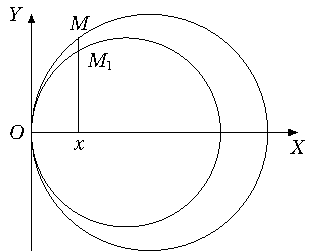
\includegraphics[scale=1]{figure/fig1-1-1.pdf}
			\caption{}\label{fig:1.1.1}
		\end{figure}
	\end{ti}